\scanpage{30}
\margin{29}
\mspage{11}
\margin{\uline{NB} les flèches $\widetilde a_i^\omega$ sont en fait superflues, cf $(37)$ et commentaires p. 19.}
\figure{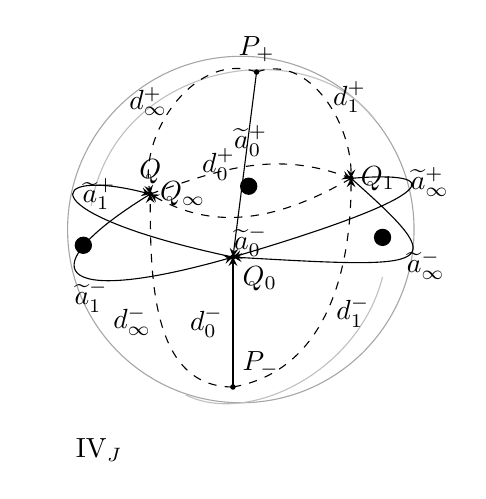
\begin{tikzpicture}[x=1cm,y=1cm,>=stealth]
\draw[gray!70] (0,0) ellipse (2.2 and 2.2);
\draw[gray!50] (-1.9,.3) .. controls (-1.6,2.1) and (.8,2.55) .. (1.7,1.4);
\draw[gray!50] (-.7,-2.1) .. controls (.1,-2.5) and (1.5,-1.8) .. (1.8,-.6);
\coordinate(P) at(.2,2);\coordinate(M) at(-.1,-2);\coordinate(A) at(-1.15,.45);\coordinate(B) at(1.4,.65);\coordinate(C) at(-.1,-.35);
\foreach \p in {P,M,A,B,C}{\fill (\p) circle(.035);}
\fill (-2,-.2) circle(.11);\fill(.1,.55) circle(.11);\fill(1.8,-.1) circle(.11);
\draw[->,dashed] (P) to[out=160,in=100] node[left]{$d_\infty^+$}(A);
\draw[->] (P)--node[left]{$d_0^+$}(C);
\draw[->,dashed] (P) to[out=20,in=90] node[right]{$d_1^+$}(B);
\draw[->,dashed] (M) to[out=180,in=270] node[left]{$d_\infty^-$}(A);
\draw[->] (M)--node[left]{$d_0^-$}(C);
\draw[->,dashed] (M) to[out=10,in=270] node[right]{$d_1^-$}(B);
\draw[->,dashed] (A) to[out=20,in=160] node[above]{$\widetilde a_0^+$}(B);
\draw[->,dashed] (B) to[out=210,in=330] node[below]{$\widetilde a_0^-$}(A);
\draw[->] (C) .. controls (-2.7,.2) and (-2.5,.8) .. (A);
\node at(-1.8,.45){$\widetilde a_1^+$};
\draw[->] (A) .. controls (-2.7,-.5) and (-2.4,-1) .. (C);
\node at(-1.9,-.85){$\widetilde a_1^-$};
\draw[->] (B) .. controls (2.6,.75) and (2.6,.45) .. (C);
\node at(2.4,.6){$\widetilde a_\infty^+$};
\draw[->] (B) .. controls (2.7,-.5) and (2.5,-.5) .. (C);
\node at(2.35,-.45){$\unsure{\widetilde a_\infty^-}$};
\node[above] at(P){$P_+$};\node[above right] at(M){$P_-$};
\node[right] at(A){$Q_\infty$};\node[right] at(B){$Q_1$};\node[below right] at(C){$Q_0$};
\node[above] at(A){$\deleted{\unsure{Q}}$};\node at(-1.8,-2.8){$\mathrm{IV}_J$};
\end{tikzpicture}}
On rajoute les \inserted{deux} sommets $\unsure{P_i^\omega|P_\infty^\omega}$ $(\omega\in\uline{\omega})$, et les flèches
\diagram{\begin{tikzcd}[ampersand replacement=\&]d_i^\omega:\quad P_\infty^\omega\arrow[r]\&Q_i\end{tikzcd}}
permutés transitivement par $G_J$, avec
\[
(34)\qquad\tau(P_{\unsure{\infty|i}}^\omega)=P_{\unsure{\infty|i}}^{\omega'},\qquad\tau(d_i^\omega)=d_i^{\omega'}
\]
Le groupoïde $\mathrm{III}_J$ est équivalent au groupoïde $\mathrm{IV}_J$ \inserted{défini par le graphe ayant} \deleted{sur} les sommets $Q_i$ $(i\in\unsure{\omega|J})$ et $P_\infty^\omega$ $(\omega\in\uline{\omega})$, les arcs $\widetilde a_i^\omega$ et $d_i^\omega$ et les \inserted{arcs} opposés, et les six relations
\[
(35)\qquad(d_{\omega'i}^\omega)^{-1}\widetilde a_{\omega i}^{\omega}d_i^\omega=1
\]
(qui impliquent d'ailleurs les relations constitutives $(16)$ pour $\mathrm{III}_J$). La donnée d'un endomorphisme de $\mathrm{IV}_J$ qui fixe les \deleted{pts} sommets (pour simplifier --- il faudra regarder aussi ceux qui permutent les sommets \inserted{$P_\omega$} en fixant les $Q_i$), \deleted{équivaut à} et qui commute à $G_J$, équivaut à la donnée des
\[
(36)\quad\left\{\begin{aligned}
u(\widetilde a_i^\omega)&=\psi_{\omega i}^\omega(\widetilde\alpha)\widetilde a_i^\omega
&\widetilde\alpha&\in\widehat\Pi_{0,3}\quad\text{(indép. de }i,\omega\text{)}\\
u(d_i^\omega)&=\psi_i^\omega(\xi)d_i^\omega\quad\bigl(=d_i^\omega\widetilde\psi_i^\omega(\xi)\bigr)
&\xi&\in\widehat\Pi_{0,3}\quad\cdots
\end{aligned}\right.
\]
\deleted{\unsure{u}}
de $\widetilde\alpha,\xi\in\widehat\Pi_{0,3}$, avec la relation déduite de $(35)$, on trouve les équations
\[
(37)\qquad\widetilde\alpha=\xi.\rho^{-1}(\xi^{-1}),
\]
i.e. $\widetilde\alpha$ est connu quand on connaît $\xi\in\widehat\Pi_{0,3}$.
\margin{il n'y a donc pas de condition sur $\xi$ ici.}
